We know that our light rays will all go to zero for $r<2M$, at $r=2m$ ``outgoing'' rays become stationary, and beyond that they can go outwards.
Our horizon is a 3-D null surface with normal vector in the r direction, and a null distance on it. This surface is a one way surface in the same way as a lightcone in flat space (once you pass through it you can't pass back out).

If we take a slice where $v=\text{const}$, then:
\begin{align*}
	d\Sigma^2 &= (2M)^2(d\theta^2 + \sin^2\theta d\phi^2)
\end{align*}
Which is a sphere of radius $2M$, so the ``Area'' is $A=16\pi M^2$.

Looking at this in terms of polar coordinates in flat spacetime, we know $r=0$ is a timelike worldline, i.e. it denotes a place in space for all times.
Looking instead at our Schwarzchild geometry, inside the Schwarzchild radius, we see:
\begin{align*}
	ds^2 (dr=0) &= -\left(1 - \frac{2M}{r}\right) dv^2 r^2 (d\theta^2 + \sin^2\theta d\phi^2)
\end{align*}
Which is always positive, and thus indicates a spacelike surface. This indicates that $r$ seems to have taken on a role more similar to a moment in time than a place in space.
Intuitively this is because there is no way for a particle to remain stationary within the Schwarzchild radius.

\subsection{Collapsing Star}
If we look at our geodesic equations for radial infall (from an infinite distance):
\begin{align*}
	r(\tau) &= \left(\frac{3}{2}\right)^\frac{2}{3} (2M)^\frac{1}{3}(\tau_* - \tau)^\frac{2}{3} \\
	t &= t_* + 2K\left[ -\frac{2}{3}\left(\frac{r}{2M}\right)^\frac{3}{2} - 2\left(\frac{r}{2M}\right)^\frac{1}{2} + \ln \frac{\sqrt{\frac{r}{2M}} +1}{\sqrt{\frac{r}{2M}} -1}\right]
\end{align*}
If we set $\tau = 0$ when $r=0$, then:
\begin{align*}
	\frac{v}{2M} &= \frac{r}{2M} - \frac{2}{3} \left(\frac{r}{2M}\right)^\frac{3}{2} + 2\ln| 1 + \sqrt{\frac{r}{2M}}|
\end{align*}
\begin{figure*}[h]
	\centering
	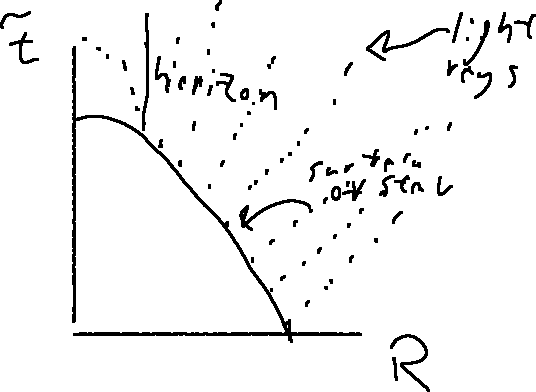
\includegraphics[width=12cm]{2-18-1.png}
	\caption*{Our collapsing star}
\end{figure*}
If we choose a proper time for our surface to go from $r=2m$ to $r0$. We say:
\begin{align*}
	r(\tau_H) &= 2M \\
	r(\tau_H) &=\left(\frac{3}{2}\right)^\frac{2}{3} (2M)^\frac{1}{3}(\tau_* - \tau_H)^\frac{2}{3} \\
	\tau_*^\frac{2}{3} &= 2M \left(\frac{3}{2}\right)^{-\frac{2}{r}} (2M)^{-\frac{1}{3}} \\
	\tau_* &= \frac{4M}{3} \\
	r(\tau_0) &= 0 \\
	0 &= \tau_* - \tau_0 \\
	\tau_0 &= \frac{4M}{3}
\end{align*}

\subsection{Redshifted light from collapsing star}
We now look at the redshift of the light coming from a collapsing star. We consider that the star emits light from the surface at fixed proper time intervals $\tau$, which is:
\begin{align*}
	\omega_* &= \frac{2\pi}{\tau}
\end{align*}
We look at what will be seen from a distant stationary observer. For this observer the proper and coordinate times are equivalent, so we look at time $t_R$ and consider the frequency the observer will observe $\omega_R(t_r) = \frac{2\pi}{\Delta t_R}$.

For ourgoing rays:
\begin{align*}
	v- 2\left(r + 2M \ln |\frac{r}{2M} -1 |\right) &= \text{const}
	v_E- 2\left(r_E + 2M \ln |\frac{r_E}{2M} -1 |\right) &= v_R- 2\left(r_R + 2M \ln |\frac{r_R}{2M} -1 |\right)
\end{align*}
Where $E$ denotes the emitter and $R$ denotes the reciever.

If we take the limit of a surface near the Schwarzchild horizon, and an extremely distant observer (and also using $t=v-r-2M\ln|\frac{r}{2M} - 1|$):
\begin{align*}
	- 4M \ln \left(\frac{r_E}{2M} -1 \right) &= t_R + r_R \\
	\frac{r_E}{2M}  -1 &= e^{-\frac{t_r - r_R}{4M}}
\end{align*}
Therefore the surface from which theobserver recieves light from, has an exponential with charactoristic time $4M$. So:
\begin{align*}
	\omega_R &= \frac{2\pi}{\Delta t_R} \\
	\omega_R &= \omega_* e^{-\frac{t_R}{4M}}
\end{align*}
Which will approach infinite redshifting with a timescale $4M$. This means that the black hole would immediately have all light become redshifting until it becomes undetectable, and therefore it suddenly appears dark.
\subsection{Kruskal coordinates}
Just like Eddington-Finkelstein coordinates, we trade our radial and temporal coordinates for new coordinates:
\begin{align*}
	U &= \sqrt{\frac{r}{2M} -1}e^{r}{4M} \cosh \frac{t}{4M} \\
	V &= \sqrt{\frac{r}{2M} - 1}e^{r}{4M} \sinh \frac{t}{4M}
\end{align*}
Outside the event horizon, and:
\begin{align*}
	U &= \sqrt{1-\frac{r}{2M}}e^{r}{4M} \sinh \frac{t}{4M} \\
	V &= \sqrt{1-\frac{r}{2M}}e^{r}{4M} \cosh \frac{t}{4M}
\end{align*}
Inside the even horizon, this gives us our line element:
\begin{align*}
	ds^2 &= \frac{32 M^3}{r} e^{-\frac{r}{2M}}(-dV^2 + dU^2) + r^2 (d\theta^2 + \sin^2\theta d\phi^2) \\
	\left(\frac{r}{2M} -1\right)e^\frac{r}{2M} &= U^2 -V^2
\end{align*}
So for lines of constant $r$ we have constant $U^2 - V^2$ and for constant $t$ we have:
\begin{align*}
	\tanh\frac{r}{4M} &= \frac{V}{U} & r &> 2M \\
	\tanh\frac{r}{4M} &= \frac{U}{V} & r &< 2M \\
\end{align*}
We say radial light rays obey:
\begin{align*}
	0 &= \frac{32 M^3}{r} e^{-\frac{r}{2M}}(-dV^2 + dU^2) \\
	V &= \pm U + \text{const}
\end{align*}
\begin{figure*}[h]
	\centering
	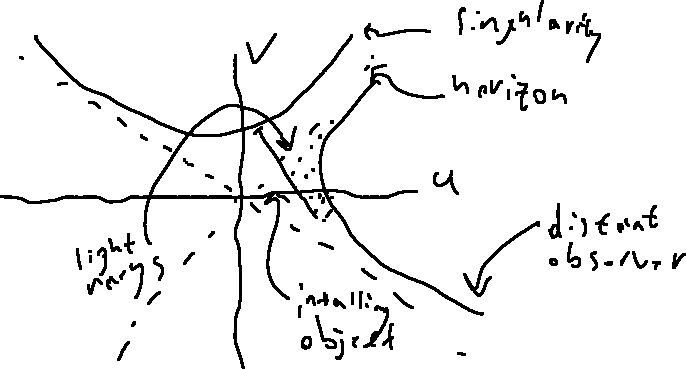
\includegraphics[width=12cm]{2-18-2.png}
	\caption*{Kruskal coordinates}
\end{figure*}
\subsection{Hand waving Hawking radiation}
Detailed calculations are outside the scope of this course, but we will look at relevant constants and come up with an argument for Hawking radiation.
If we consider the energy carried away by particles generated near the horizon then we consider the energy the black hole must lose to obey conservation of energy.
If we give our particle $\bm{p}$ four momentum, and it's pair particle $\tilde{\bm{p}}$ four momentum. If we consider the energy conservation driven by $\xi$ we see:
\begin{align*}
	\bm{\xi}\cdot\bm{p} + \bm{\xi}\cdot\tilde{\bm{p}} &= 0 \\
	\bm{\xi}\cdot\bm{\xi} &= 1 -\frac{2M}{r}
\end{align*}
So $\xi$ is timelike outside the horizon and spacelike inside it. Outside the horizen we have $-\bm{xi}\cdot\bm{p} >0$, which corresponds to the energy measured by an observer with a 4-velocity parrallel to our killing vector.
Inside the horizon $-\bm{\xi}\cdot\tilde{\bm{p}}$, this will become a momentum like term (because the role of the $t$ coordinate has flipped) and therefore it could be negative. We now look at the rate of change the black hole loses energy.
We start by saying that the rate should be proportional to $\hbar$, which has an associated length scale $l_p = \sqrt{\frac{G\hbar}{c^3}}$. We then say that this rate should look something like:
\begin{align*}
	\frac{dM}{dt} &= -\nu \frac{\hbar}{M^2}
\end{align*}
Where $\nu$ is a constant derived from QFT, but we find that this is going to be related to $\frac{\hbar}{8\pi M} = k_B T$
\begin{align*}
	M(t) &= \left[3\nu\hbar(t_* -t)\right]^\frac{1}{3}
\end{align*}
Which gives us an evaporation time $\tau \approx \frac{1}{3\nu}\frac{M^3}{\hbar}$ which is approximately $8.3 \times 10^{-26} \left(\frac{M}{1 g}\right)^3 s$
\section{Rotation}
When we say we are looking at slow rotation, we mean that our corrections should be only first order in angular velocity. Centripital accelerations then includes second order corrections.

This will allow us to see that the motion of this mass will change the curvature of the space. We call these gravito-magnetic effects.
\subsection{Slow Rotation in Schwarzchild geometry}
We consider test gyroscopes in order to probe spacetime. We can see our geodesics give us:
\begin{align*}
	\frac{d u^\alpha}{d\tau} &= -\Gamma_{\beta\gamma}^\alpha u^\beta u^\gamma
\end{align*}
In addition to our four velocity we also give our test gyroscope a spin vector, which is a spacelike vector $\bm{S}$. In a local inertial frame we can say:
\begin{align*}
	S^\alpha &= (0,\bm{S}) \\
	S_\alpha u^\alpha &= 0
\end{align*}
And our total spin is a constant of motion. In flat spacetime we should have:
\begin{align*}
	\frac{dS^\alpha}{d\tau} &= 0
\end{align*}
While in general we want it to obey everything we just said in local inertial components. We also want it to be linear in the components of our spin, and maintain the same form in all coordinate systems. Therefore we find:
\begin{align*}
	\frac{dS^\alpha}{d\tau} + \Gamma^\alpha_{\beta\gamma} S^\beta u^\gamma &= 0
\end{align*}
